\chapter{Development Timeline}

The development timelines shown in Figures 12.1, 12.2, and 12.3 depict a set of tasks that need to be completed throughout the year.  A Gantt Chart is used to break down our project into smaller deliverables.  Each chart corresponds to an individual academic school quarter.

\begin{figure}[!h]
	\centering
	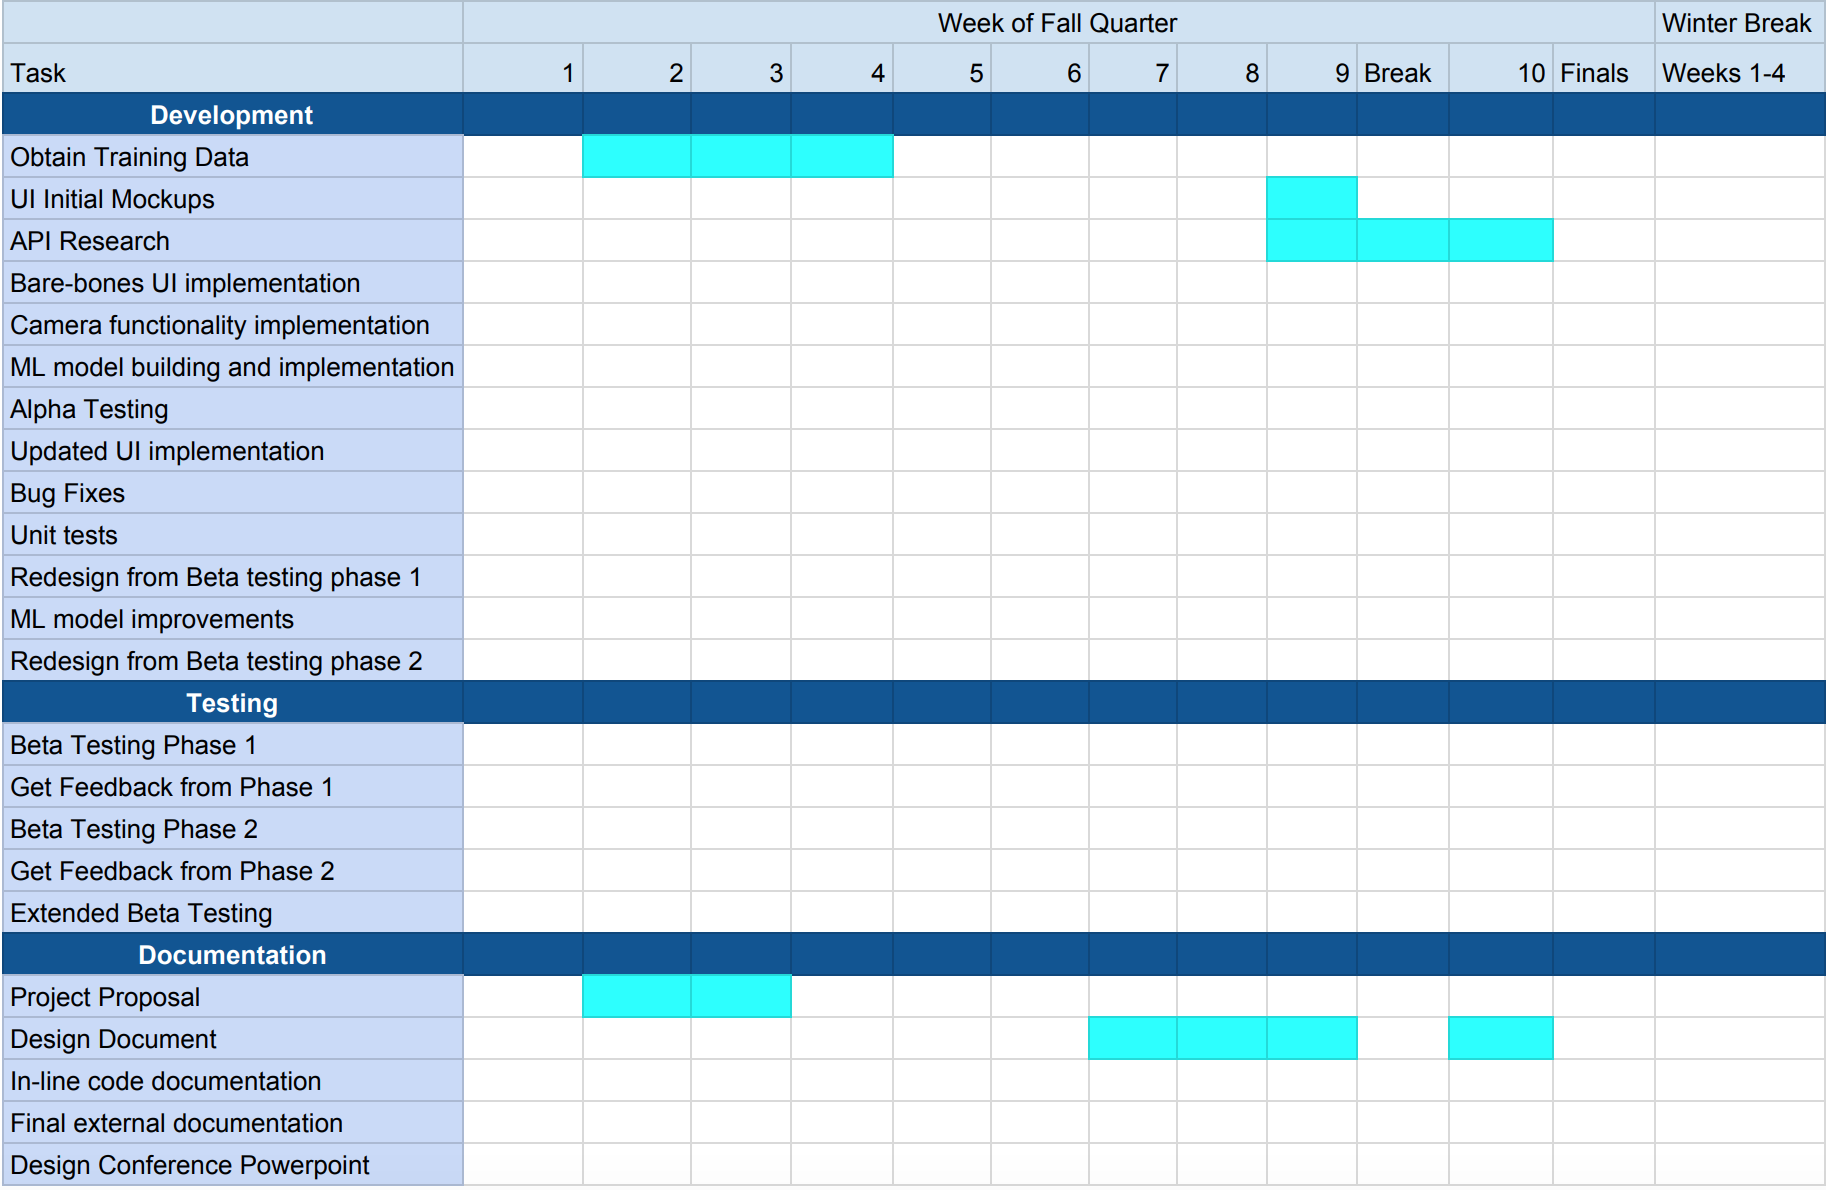
\includegraphics[width=1\textwidth]{timeline1}
	\caption{Fall Quarter Development Timeline}
	\label{fig:timeline1}
\end{figure}

\begin{figure}[!h]
	\centering
	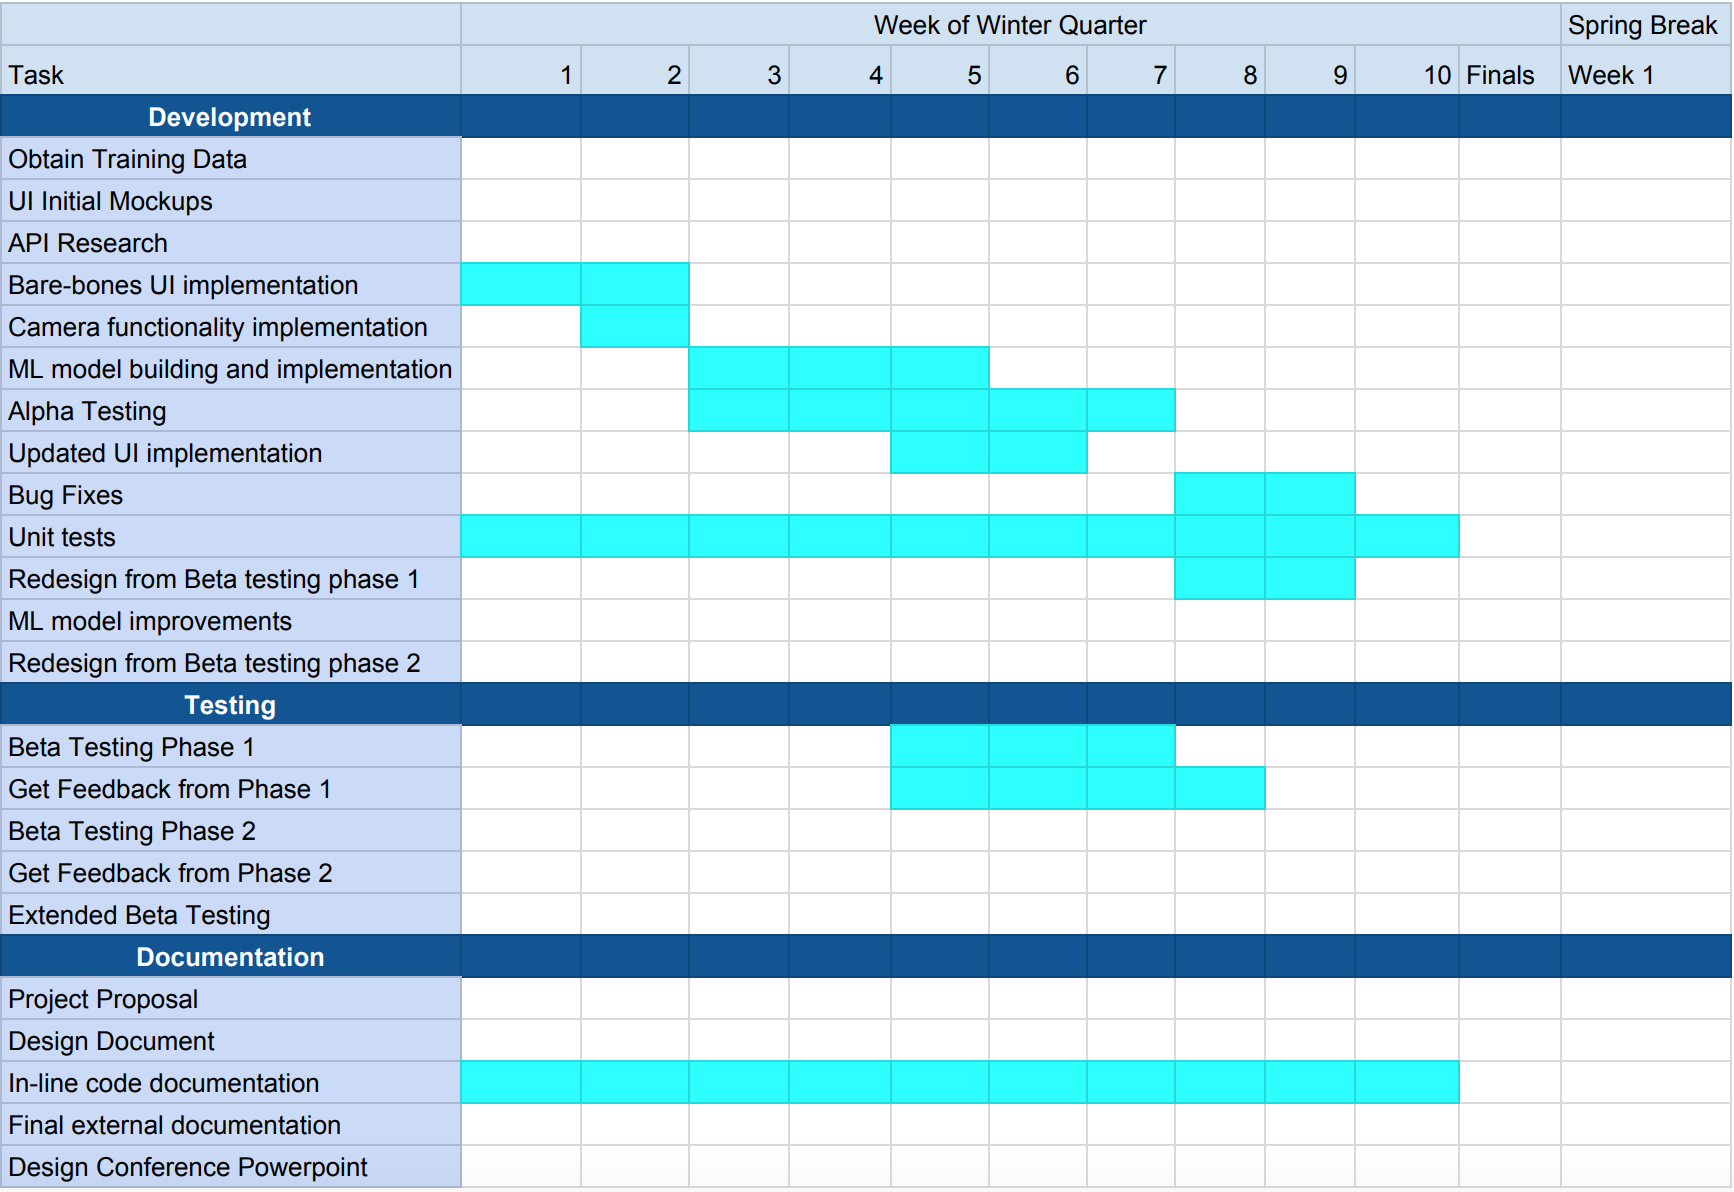
\includegraphics[width=1\textwidth]{timeline2}
	\caption{Winter Quarter Development Timeline}
	\label{fig:timeline2}
\end{figure}

\begin{figure}[!h]
	\centering
	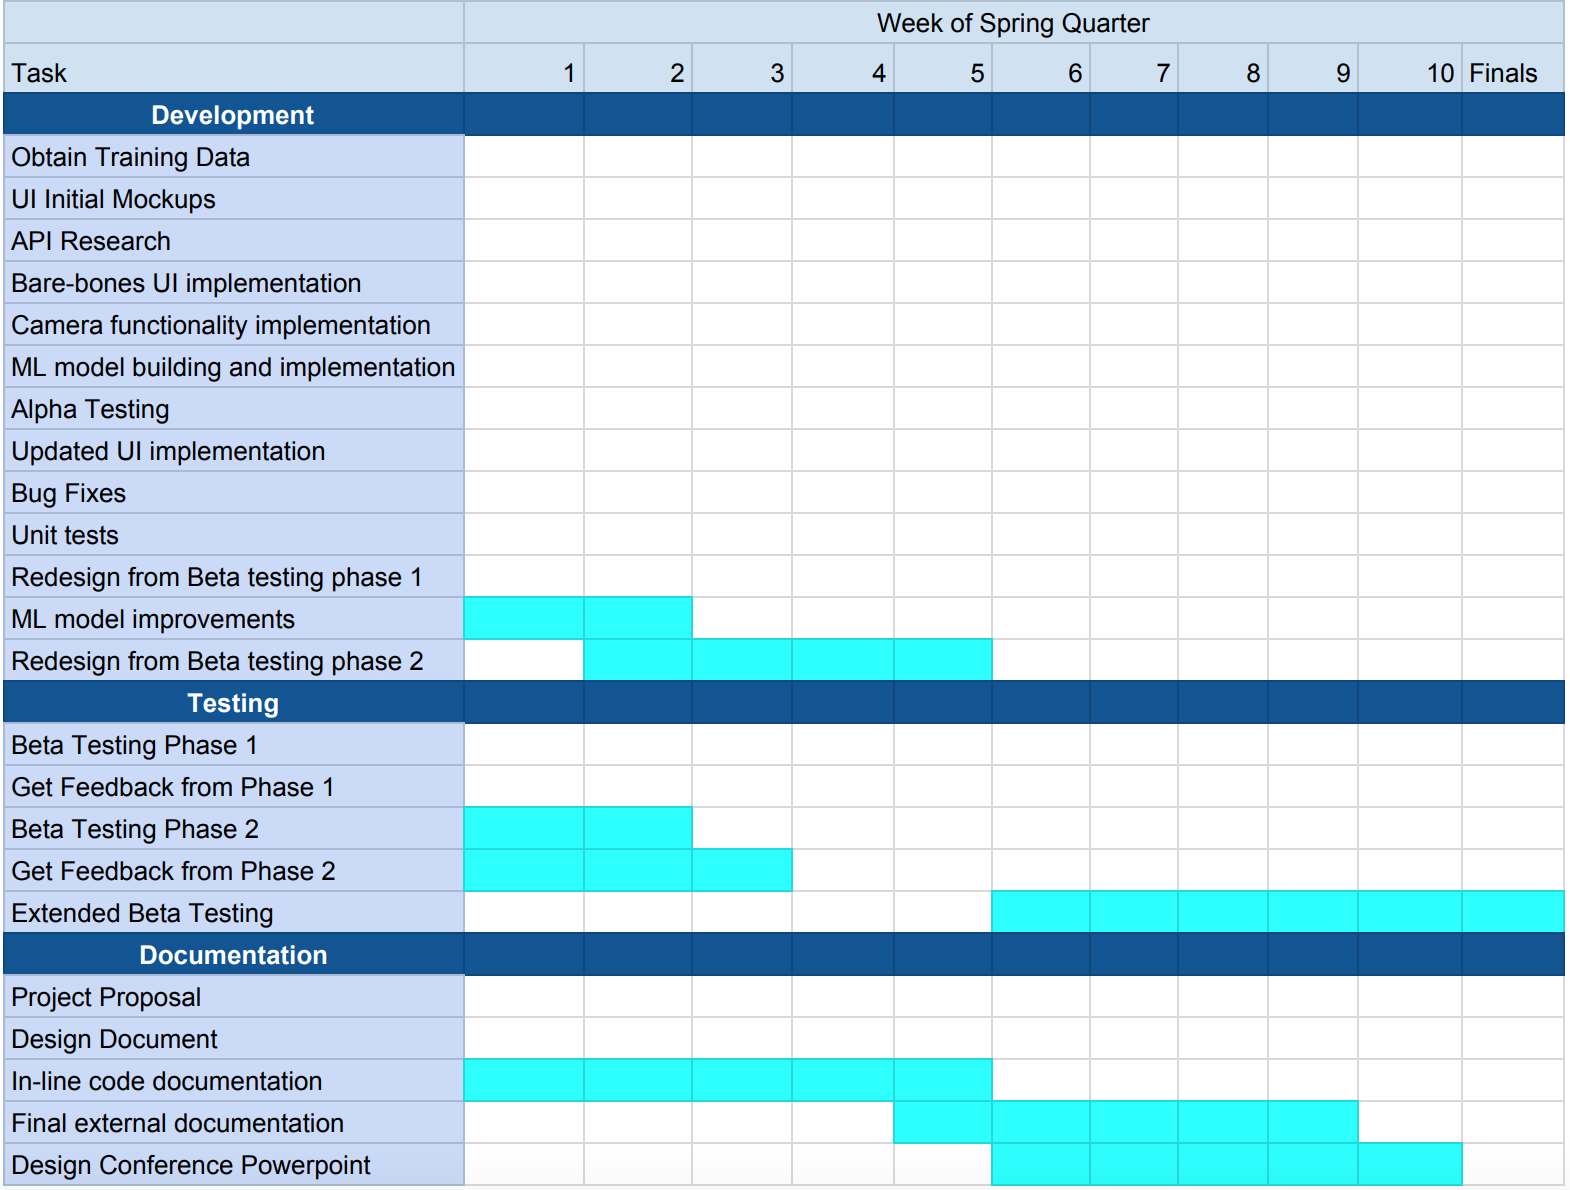
\includegraphics[width=1\textwidth]{timeline3}
	\caption{Spring Quarter Development Timeline}
	\label{fig:timeline3}
\end{figure}